\documentclass[a4paper, 12pt]{scrartcl}
\usepackage[ngerman]{babel}
\usepackage[utf8]{inputenc}
\usepackage[T1]{fontenc}
\usepackage{lmodern}

\linespread{1.2}
\parindent0cm
\usepackage{graphicx}
\usepackage{hyperref}
\usepackage{float}
\usepackage{tabularx}
\usepackage{multicol}
\usepackage{units}

\usepackage{listings}
\usepackage{color}
\usepackage{geometry}
	\geometry{a4paper, top=25mm, left=20mm, right=20mm, bottom=30mm, headsep=10mm, footskip=12mm}
\usepackage{amssymb}
	

\lstset{literate=%
	{Ö}{{\"O}}1
	{Ä}{{\"A}}1
	{Ü}{{\"U}}1
	{ü}{{\"u}}1
	{ä}{{\"a}}1
	{ö}{{\"o}}1
	{█}{{$\blacksquare$}}1
	{~}{{\textasciitilde}}1
}

\definecolor{mygreen}{rgb}{0,0.6,0}
\definecolor{mygray}{rgb}{0.5,0.5,0.5}
\definecolor{mymauve}{rgb}{0.58,0,0.82}
\definecolor{deepred}{rgb}{0.6,0,0}

\lstset{ %
	backgroundcolor=\color{white},   % choose the background color; you must add \usepackage{color} or \usepackage{xcolor}; should come as last argument
	basicstyle=\footnotesize,        % the size of the fonts that are used for the code
	breakatwhitespace=false,         % sets if automatic breaks should only happen at whitespace
	breaklines=true,                 % sets automatic line breaking
	captionpos=b,                    % sets the caption-position to bottom
	commentstyle=\color{mygreen},    % comment style
	deletekeywords={...},            % if you want to delete keywords from the given language
	escapeinside={\%*}{*)},          % if you want to add LaTeX within your code
	extendedchars=true,              % lets you use non-ASCII characters; for 8-bits encodings only, does not work with UTF-8
	frame=single,	                 % adds a frame around the code
	keepspaces=true,                 % keeps spaces in text, useful for keeping indentation of code (possibly needs columns=flexible)
	keywordstyle=\color{blue},       % keyword style
	language=Python,                 % the language of the code
	morekeywords={*,...},            % if you want to add more keywords to the set
	emph={makevideo,checkgreen,checkblue,lenken,line,linienfahren,main},
	emphstyle=\color{deepred},
	numbers=left,                    % where to put the line-numbers; possible values are (none, left, right)
	numbersep=5pt,                   % how far the line-numbers are from the code
	numberstyle=\tiny\color{mygray}, % the style that is used for the line-numbers
	rulecolor=\color{black},         % if not set, the frame-color may be changed on line-breaks within not-black text (e.g. comments (green here))
	showspaces=false,                % show spaces everywhere adding particular underscores; it overrides 'showstringspaces'
	showstringspaces=false,          % underline spaces within strings only
	showtabs=false,                  % show tabs within strings adding particular underscores
	stepnumber=2,                    % the step between two line-numbers. If it's 1, each line will be numbered
	stringstyle=\color{mymauve},     % string literal style
	tabsize=2,	                     % sets default tabsize to 2 spaces
	title=\lstname                   % show the filename of files included with \lstinputlisting; also try caption instead of title
}
 
\begin{document}

\section{import}
\lstinputlisting[language=Python,firstline=1,lastline=14]{../main.py}

Am Anfang der Hauptdatei werden die benötigten Module importiert, gefolgt von den beiden ausgelagerten Dateien. Von aufrauemen.py werden nur die benötigten Funktionen importiert, von setup.py wird alles importiert, da diese Datei keine Funktion enthält.

In den Zeilen $10$ bis $14$ werden die benötigten Einstellungen für OpenCV 2 vorgenommen und ein erstes Bild aufgenommen.

\section{makevideo}
\lstinputlisting[language=Python,firstline=17,lastline=33]{../main.py}

Die Aufgabe der \textit{makevideo} Funktion ist es die von der Kamera aufgenommenen Bilder als ein Video zu exportieren. Da das Video nur zur Fehleranalyse und Veranschaulichung dient, wird es vernachlässigt ob das Video in Echtzeit läuft. Dafür wird die aktuelle Fahrzeit, ab dem erkennen der grünen Ampel unten links im Bild eingeblendet. Außerdem wird der zu dem Bild gehörende Messpunkt und dessen Wert eingezeichnet.

Das Video in Zusammenhang mit den eingeblendeten Werten ermöglicht eine deutlich bessere Fehleranalyse als eine Textausgabe über die Konsole (Abb.: \ref{schuh_im_bild}).

\begin{figure}[ht!] \centering
	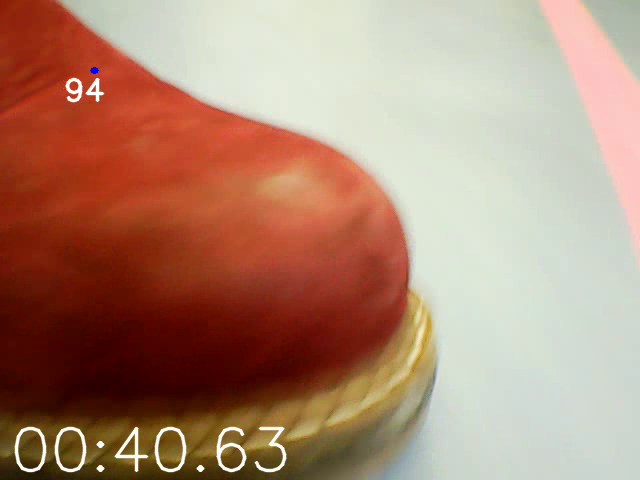
\includegraphics[width=.5\textwidth]{schuh_im_bild.png}
	\caption{Kamerabild mit Zeitanzeige und Messpunkt, abgelenkt von einem roten Schuh}
	\label{schuh_im_bild}
\end{figure}

\section{checkgreen}
\lstinputlisting[language=Python,firstline=36,lastline=50]{../main.py}

\section{checkblue}
\lstinputlisting[language=Python,firstline=53,lastline=73]{../main.py}

\section{lenken}
\lstinputlisting[language=Python,firstline=76,lastline=101]{../main.py}

\section{line}
\lstinputlisting[language=Python,firstline=104,lastline=119]{../main.py}

\section{linienfahren}
\lstinputlisting[language=Python,firstline=122,lastline=164]{../main.py}

\section{main}
\lstinputlisting[language=Python,firstline=167,lastline=217]{../main.py}

\section{main.py}
\lstinputlisting[language=Python]{../main.py}

\section{setup.py}
\lstinputlisting[language=Python]{../setup.py}

\section{aufraeumen.py}
\lstinputlisting[language=Python]{../aufraeumen.py}




\end{document}
